\documentclass{article}
\usepackage[utf8]{inputenc}
\usepackage{hyperref}
\usepackage[letterpaper, portrait, margin=1in]{geometry}
\usepackage{enumitem}
\usepackage{amsmath}
\usepackage{booktabs}
\usepackage{graphicx}
\usepackage{float}

\usepackage{hyperref}
\hypersetup{
colorlinks=true,
    linkcolor=black,
    filecolor=black,      
    urlcolor=blue,
    citecolor=black,
}
\usepackage{natbib}

\usepackage{titlesec}
  
\title{Homework 3}
\author{Lin Yang}
\date{\today}
  
\begin{document}
\maketitle  
\section{Python or Stata}
$y_i = e^\alpha \delta^{d_i} z_i^\gamma e^{\eta_i}$
~\\
(a) Show that $ln(y_i) = \alpha + ln(\delta) d_i+ \gamma ln(z_i) + \eta_i$

~\\
Taking natural log transformation on the both sides: 

$$ln(y_i) = \alpha ln(e) + d_i ln(\delta) + \gamma ln(z_i) + \eta_i ln(e)$$

$$ln(y_i) = \alpha + ln(\delta) d_i  + \gamma ln(z_i) + \eta_i$$

~\\
(b) Intuitive interpretation of $\delta$:

 On the average, the household who received a retrofit has $\delta$ unit less of electricity use when compared to a non-retrofit household. 


~\\
(c) Show that $\frac{\Delta y_i}{\Delta d_i} = \frac{\delta-1}{\delta^{d_i}}y_i$. \\
\begin{equation}
\begin{split}
\frac{\Delta y_i}{\Delta d_i} &= \frac{e^\alpha \delta^{(d_i =1)} z_i^\gamma e^{\eta_i}- e^\alpha \delta^{(d_i =0)} z_i^\gamma e^{\eta_i}}{(d_i =1)-(d_i =0)}\\
	&= e^\alpha \delta z_i^\gamma e^{\eta_i}- e^\alpha  z_i^\gamma e^{\eta_i} \\ &=(\delta-1)e^\alpha  z_i^\gamma e^{\eta_i} \\
		 &= \frac{(\delta-1)}{\delta^{d_i} } e^\alpha  z_i^\gamma e^{\eta_i} \delta^{d_i}\\
		  &= \frac{(\delta-1)}{\delta^{d_i} } y_i
\end{split}
\end{equation}

Intuitive interpretation of $\frac{\Delta y_i}{\Delta d_i} $ is for each household, the amount of electricity use change from participating into retrofit program versus not participating. 

~\\
(d) Show that $\frac{\alpha y_i}{\alpha z_i} = \gamma \frac{y_i}{z_i}$. \\

\begin{equation}
\begin{split}
\frac{\alpha y_i}{\alpha z_i} &= \gamma  z_i^{\gamma-1} e^\alpha \delta^{d_i}  e^{\eta_i}\\
	&= \gamma \frac{e^\alpha \delta^{d_i} z_i^\gamma e^{\eta_i}}{z_i}\\
	&=\gamma \frac{y_i}{z_i}
\end{split}
\end{equation}

Intuitive interpretation of $\frac{\alpha y_i}{\alpha z_i}$ is for each household, the amount of electricity use change by one unit change of the size of the home in square feet. 

~\\
(e)
Estimate the log-transformed equation via ordinary least squares on the transformed parameters using any algorithm you would like. A table including the coefficient estimates, the average marginal effects estimates and Bootstrap the 95\% confidence intervals.

\begin{table}[H]
	\centering
	\begin{tabular}{lll}
\toprule
{} &      Coefficients & Average Marginal Effects \\
{} & (95\% Bootsrap CI) &       (95\% Bootstrap CI) \\
\midrule
Retrofit &             -0.10 &                  -113.98 \\
         &    (-0.12, -0.09) &        (-182.14, -53.88) \\
lnSqft   &              0.89 &                     0.63 \\
         &      (0.88, 0.91) &             (0.49, 0.79) \\
lnTemp   &              0.28 &                     4.00 \\
         &      (0.04, 0.52) &             (1.62, 5.68) \\
Constant &             -0.77 &                    -0.77 \\
         &     (-1.84, 0.28) &            (-1.84, 0.28) \\
\bottomrule
\end{tabular}
	
	\caption{OLS Regression Coefficients Estimates and Average Marginal Effects with 95\% confidence intervals bootstrapped using 1,000 replications}
\end{table}

~\\
(f)
Graph the average marginal effects of outdoor temperature and square feet of the home with bands for their bootstrapped confidence intervals so that they are easy to interpret and compare. 
\begin{figure}[ht]
\centering
	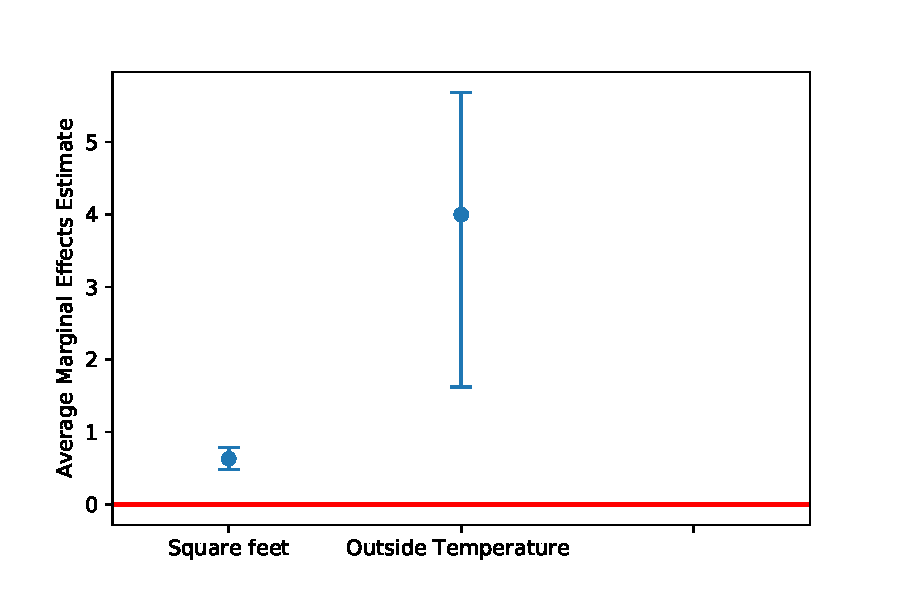
\includegraphics[scale = 0.9]{hw3f.pdf}
    \caption{Average Marginal Effects of Square feet and Outdoor Temperature with 95\% confidence intervals bootstrapped using 1,000 replications}

\end{figure}











\end{document}

